\documentclass[12pt,fleqn]{article}\usepackage{../../common}
\begin{document}
Katı-Gövde Simülasyonu

Bir örnek gövde üzerinde simülasyon yapmaya uğraşalım. Elimizde bir simit, ya da
geometride torus denen bir şekil var. Bu dosya STL denen bir format içinde,
detaylar için [1]. Torus STL şekli içiçe geçmiş üçgenler ile tanımlı, bu
üçgenlerin herbirine dik olan normal vektörü biliyoruz. O üçgenlerden birinin
orta noktasından çıkan vektörlerden birini ters çevirirsek, o noktaya o yönde
bir kuvvet uyguladığımızı hayal edelim, ve simülasyonun geri kalanını bu
noktadan devam ettirelim.

\begin{minted}[fontsize=\footnotesize]{python}
import matplotlib.pyplot as plt
from mpl_toolkits import mplot3d
import pandas as pd, numpy as np
from stl import mesh

your_mesh = mesh.Mesh.from_file('torus.stl')

prop = your_mesh.get_mass_properties()
print ('\nhacim',prop[0])
print ('\nyercekim merkezi (COG)',prop[1])
print ('\nCOG noktasinda atalet matrisi')
print (prop[2])

fig = plt.figure()
axes = mplot3d.Axes3D(fig)

scale = your_mesh.points.flatten()
axes.add_collection3d(mplot3d.art3d.Poly3DCollection(your_mesh.vectors,alpha=0.3))
axes.auto_scale_xyz(scale, scale, scale)

def plot_vector(fig, orig, v, color='blue'):
   ax = fig.gca(projection='3d')
   orig = np.array(orig); v=np.array(v)
   ax.quiver(orig[0], orig[1], orig[2], v[0], v[1], v[2],color=color)
   ax = fig.gca(projection='3d')  
   return fig

LIM = 5
axes.set_xlim(-LIM,LIM);axes.set_ylim(-LIM,LIM);axes.set_zlim(-LIM,LIM)

SCALE = 4
tidx = 2000
o = np.mean(your_mesh.vectors[tidx],axis=0)
axes.plot (o[0],o[1],o[2],'gd')
n = your_mesh.get_unit_normals()[tidx]
plot_vector(fig, o, n*SCALE)
plot_vector(fig, o, -n*SCALE, color='red')
axes.view_init(azim=84,elev=28)

plt.savefig('phy_005_basics_04_05.png')
\end{minted}

\begin{verbatim}

hacim 4.917547323463467

yercekim merkezi (COG) [-1.57676116e-12  3.04791724e-11 -6.76980205e-11]

COG noktasinda atalet matrisi
[[ 3.22258484e+00 -5.48156069e-10  2.81815519e-10]
 [-5.48156069e-10  3.22258489e+00  2.90733626e-09]
 [ 2.81815519e-10  2.90733626e-09  5.83209197e+00]]
\end{verbatim}

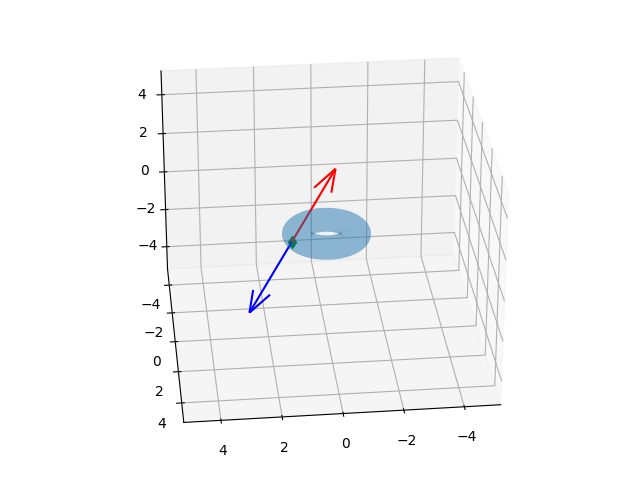
\includegraphics[width=20em]{phy_005_basics_04_05.png}





[devam edecek]

Kaynaklar

[1] Bayramli, {\em 3D Baskıya Hazır CAD Tasarımlarına Erişmek, Numpy-STL},
    \url{https://burakbayramli.github.io/dersblog/sk/2020/08/numpy-stl.html}

[2] Witkin, {\em Physically Based Modeling}

\end{document}



